\uuid{spB4}
\exo7id{5102}
\titre{exo7 5102}
\auteur{rouget}
\organisation{exo7}
\datecreate{2010-06-30}
\isIndication{false}
\isCorrection{true}
\chapitre{Continuité, limite et étude de fonctions réelles}
\sousChapitre{Etude de fonctions}
\module{Analyse}
\niveau{L1}
\difficulte{}

\contenu{
\texte{
Construire le graphe des fonctions suivantes~:
}
\begin{enumerate}
    \item \question{(*) $f_1(x)=2|2x-1|-|x+2|+3x$.}
\reponse{$f_1$ est définie et continue sur $\Rr$, dérivable sur $\Rr\setminus\left\{-2,\frac{1}{2}\right\}$. On précise dans
un tableau l'expression de $f_1(x)$ suivant les valeurs de $x$.

$$
\begin{array}{|c|lcc|ccc|ccr|}
\hline
x&-\infty& &\multicolumn{2}{c}{-2}& &\multicolumn{2}{c}{1/2}& &+\infty\\
\hline
|2x-1|& &-2x+1& & &-2x+1& & &2x-1& \\
\hline
|x+2|& &-x-2& & &x+2& & &x+2& \\
\hline
f_1(x)& &4& & &-2x& & &6x-4& \\
\hline
\end{array}
$$
On en déduit $\mathcal{C}_1$.


$$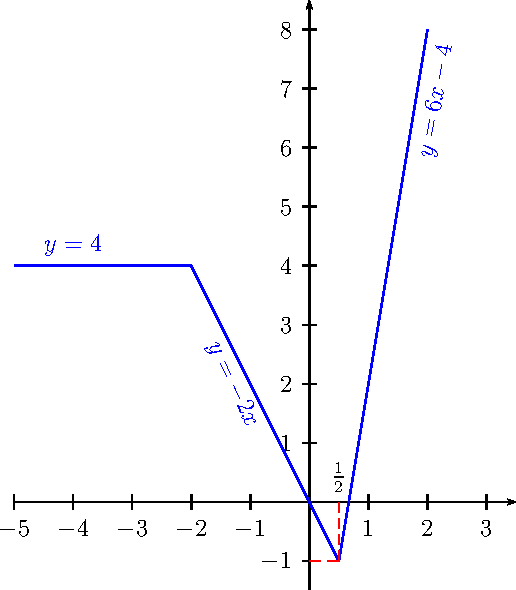
\includegraphics{../images/img005102-1}$$}
    \item \question{(**) $f_{2}(x)=\ln(\ch x)$.}
\reponse{Soit $x\in\Rr$. $\ch x\geq1$ et donc $f_2(x)$ existe et $f_2(x)\geq0$. $f_2$ est donc définie sur $\Rr$. De
plus, $f_2$ est continue et dérivable sur $\Rr$, paire.
Puisque la fonction $x\mapsto\ch x$ est strictement croissante sur $\Rr^+$ à valeurs dans $]0,+\infty[$ et que la fonction $x\mapsto\ln x$ est
strictement croissante sur $]0,+\infty[$, $f_2$ est strictement croissante sur $\Rr^+$ et, par parité, strictement
décroissante sur $\Rr^-$.
$f_2$ est paire et donc $f_2'$ est impaire. Par suite, $f_2'(0)=0$ et $\mathcal{C}_2$ admet l'axe des abscisses pour
tangente en $(0,f_2(0))=(0,0)$.
\textbf{Etude en} $+{\infty}$. Pour $x\geq0$,

$$f_2(x)=\ln\left(\frac{1}{2}(e^x+e^{-x}))=\ln(e^x+e^{-x}\right)-\ln2=\ln(e^x(1+e^{-2x}))-\ln2=x-\ln2+\ln(1+e^{-2x}).$$
Quand $x$ tend vers $+\infty$, $e^{-2x}$ tend vers $0$ et donc, $\ln(1+e^{-2x})$ tend vers $0$. On en déduit que
$\lim_{x\rightarrow +\infty}f_2(x)=+\infty$. De plus, $\lim_{x\rightarrow +\infty}(f_2(x)-(x-\ln2))=0$ et la droite $(D)$ d'équation
$y=x-\ln2$ est asymptote à $\mathcal{C}_2$ en $+\infty$. Par symétrie par rapport à la droite $(Oy)$, la droite $(D')$ d'équation $y=-x-\ln2$ est asymptote à $\mathcal{C}_2$ en $-\infty$. Enfin, pour tout réel $x$,

$$f_2(x)-(x-\ln2)=\ln(1+e^{-2x})>\ln1=0,$$
et $\mathcal{C}_2$ est strictement au-dessus de $(D)$ sur $\Rr$. De même, $\mathcal{C}_2$ est strictement au-dessus de
$(D')$ sur $\Rr$.
On en déduit $\mathcal{C}_2$.


$$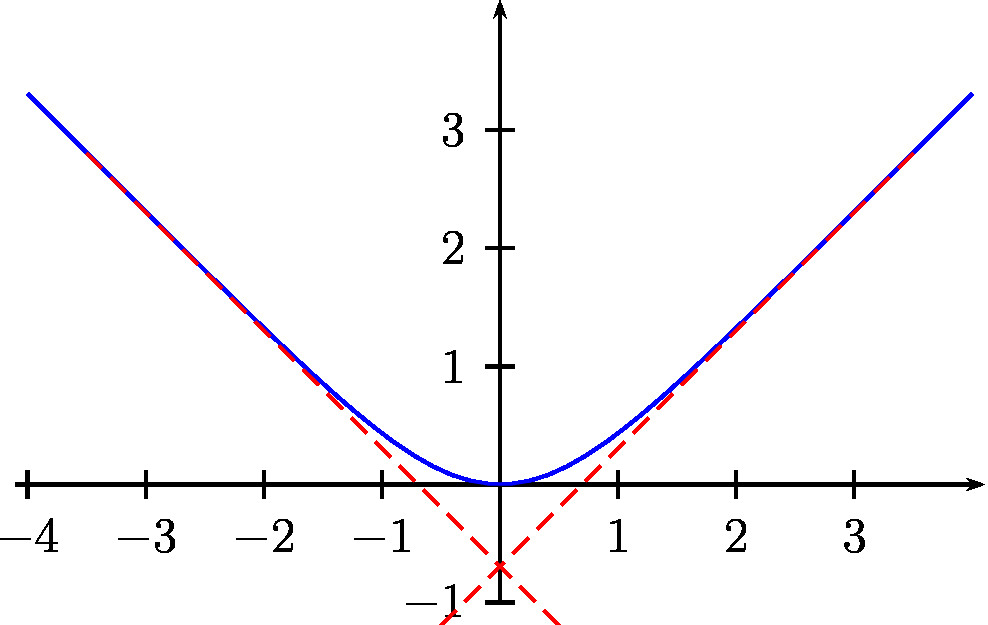
\includegraphics{../images/img005102-2}$$}
    \item \question{(***) $f_3(x)=x+\sqrt{|x^2-1|}$.}
\reponse{$f_3$ est définie et continue sur $\Rr$, dérivable sur $\Rr\setminus\{-1,1\}$.
\textbf{Etude en} $-\infty$. Soit $x\leq-1$.

$$f_3(x)=x+\sqrt{x^2-1}=\frac{(x+\sqrt{x^2-1})(x-\sqrt{x^2-1})}{x-\sqrt{x^2-1}}=\frac{1}{x-\sqrt{x^2-1}}.$$
Or, quand $x$ tend vers $-\infty$, $x-\sqrt{x^2-1}$ tend vers $-\infty$ et donc $\lim_{x\rightarrow -\infty}f_3(x)=0$.
\textbf{Etude en} $+\infty$. Immédiatement, $\lim_{x\rightarrow +\infty}f_3(x)=+\infty$. Ensuite, pour $x\geq1$,

$$\frac{f_3(x)}{x}=\frac{x+\sqrt{x^2-1}}{x}=1+\sqrt{1-\frac{1}{x^2}},$$
qui tend vers $2$ quand $x$ tend vers $+\infty$. Mais alors,

$$f_3(x)-2x=-x+\sqrt{x^2-1}=\frac{(-x+\sqrt{x^2-1})(-x-\sqrt{x^2-1})}{-x-\sqrt{x^2-1}}=-\frac{1}{x+\sqrt{x^2-1}}.$$
On en déduit que $\lim_{x\rightarrow +\infty}(f_3(x)-2x)=0$ et donc que la droite $(D)$ d'équation $y=2x$ est asymptote à $\mathcal{C}_3$ en $+\infty$.
\textbf{Etude en} $1$. Pour $x>1$,

$$\frac{f_3(x)-f_3(1)}{x-1}=\frac{(x-1)+\sqrt{(x-1)(x+1)}}{x-1}=1+\sqrt{\frac{x+1}{x-1}},$$
et pour $x\in]-1,1[$,

$$\frac{f_3(x)-f_3(1)}{x-1}=\frac{(x-1)+\sqrt{(-x+1)(x+1)}}{-(-x+1)}=1-\sqrt{\frac{x+1}{-x+1}}.$$
Par suite, $\lim_{x\rightarrow 1,\;x>1}\frac{f_3(x)-f_3(1)}{x-1}=+\infty$ et
$\lim_{x\rightarrow 1,\;x<1}\frac{f_3(x)-f_3(1)}{x-1}=-\infty$. On en déduit que $f_3$ n'est pas dérivable en $1$, mais que
$\mathcal{C}_3$ admet deux demi-tangentes parallèles à $(Oy)$ au point de $\mathcal{C}_3$ d'abscisse $1$. Les résultats
sont analogues en $-1$.
\textbf{Etude des variations de} $\bf{f_3}$. Pour $x\in]-\infty,-1[\cup]1,+\infty[$, $f_3(x)=x+\sqrt{x^2-1}$ et donc

$$f_3'(x)=1+\frac{x}{\sqrt{x^2-1}}=\frac{x+\sqrt{x^2-1}}{\sqrt{x^2-1}}.$$

Si $x>1$, on a $x+\sqrt{x^2-1}>0$ et donc, $f_3'(x)>0$. Si $x<-1$, on a

$$\sqrt{x^2-1}<\sqrt{x^2}=|x|=-x,$$
et donc, $x+\sqrt{x^2-1}<0$ puis $f_3'(x)<0$. Ainsi, $f_3$ est strictement décroissante sur $]-\infty,-1[$ et
strictement croissante sur $]1,+\infty[$.
Pour $x\in]-1,1[$, $f_3(x)=x+\sqrt{-x^2+1}$ et donc

$$f_3'(x)=1-\frac{x}{\sqrt{-x^2+1}}=\frac{\sqrt{-x^2+1}-x}{\sqrt{-x^2+1}}.$$
Si $x\in]-1,0]$, on a clairement $f_3'(x)>0$. Si x$\in[0,1[$, par stricte croissance de la fonction $x\mapsto x^2$ sur $\Rr^+$, on a

$$\mbox{sgn}(f_3'(x))=\mbox{sgn}(\sqrt{-x^2+1}-x)=\mbox{sgn}((-x^2+1)-x^2)=\mbox{sgn}(1-2x^2)=\mbox{sgn}((1-x\sqrt{2})
(1+x\sqrt{2}))=\mbox{sgn}[\frac{1}{\sqrt{2}}-x).$$
Donc, $f_3'$ est strictement positive sur $\left[0,\frac{1}{\sqrt{2}}\right[$, strictement négative sur $\left]\frac{1}{\sqrt{2}},1\right[$
et s'annule en $\frac{1}{\sqrt{2}}$.
En résumé, $f_3'$ est strictement négative sur $]-\infty,-1[$ et sur $\left]\frac{1}{\sqrt{2}},1\right[$ et strictement positive
sur $\left]-1,\frac{1}{\sqrt{2}}\right[$ et sur $]1,+\infty[$. $f_3$ est donc strictement croissante sur $]-\infty,-1]$ et sur
$\left[\frac{1}{\sqrt{2}},1\right[$ et strictement décroissante sur $\left[-1,\frac{1}{\sqrt{2}}\right]$ et sur $[1,+\infty[$.
On en déduit $\mathcal{C}_3$.

$$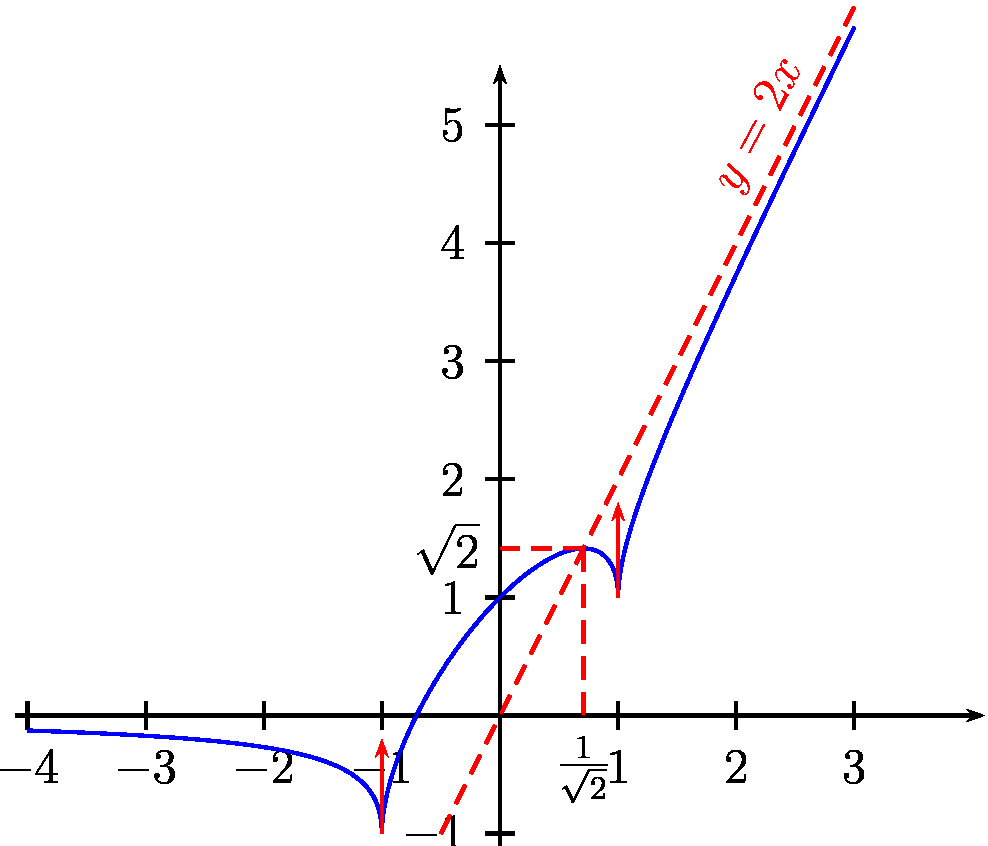
\includegraphics{../images/img005102-3}$$}
    \item \question{(**) $f_4(x)=|\tan x|+\cos x$.}
\reponse{$f_4$ est définie sur $\Rr\setminus\left(\frac{\pi}{2}+\pi\Zz\right)$, $2\pi$-périodique et paire. On étudie
donc $f_4$ sur $\left[0,\frac{\pi}{2}\right[\cup\left]\frac{\pi}{2},\pi\right]$.
\textbf{Etude des variations de} $\bf{f_4}$. Pour $x\in\left[0,\frac{\pi}{2}\right[$, $f_4(x)=\tan x+\cos x$ et donc,

$$f_4'(x)=\frac{1}{\cos^2x}-\sin x\geq 1-1=0,$$
avec égalité si et seulement si $\sin x=\cos^2x=1$ ce qui est impossible. Donc, $f_4'$ est strictement positive sur
$\left[0,\frac{\pi}{2}\right[$ et $f_4$ est strictement croissante sur $\left[0,\frac{\pi}{2}\right[$.
Pour $x\in\left]\frac{\pi}{2},\pi\right]$, $f_4(x)=-\tan x+\cos x$ et $f_4$ est strictement décroissante sur
$\left]\frac{\pi}{2},\pi\right]$ en tant que somme de deux fonctions strictement décroissantes sur $\left]\frac{\pi}{2},\pi\right]$.
On a immédiatement
$\displaystyle\lim_{\substack{x\rightarrow\frac{\pi}{2}\\
x<\frac{\pi}{2}}}f_4(x)=\displaystyle\lim_{\substack{x\rightarrow\frac{\pi}{2}\\
x>\frac{\pi}{2}}}f_4(x)=+\infty$.
On en déduit $\mathcal{C}_4$.

$$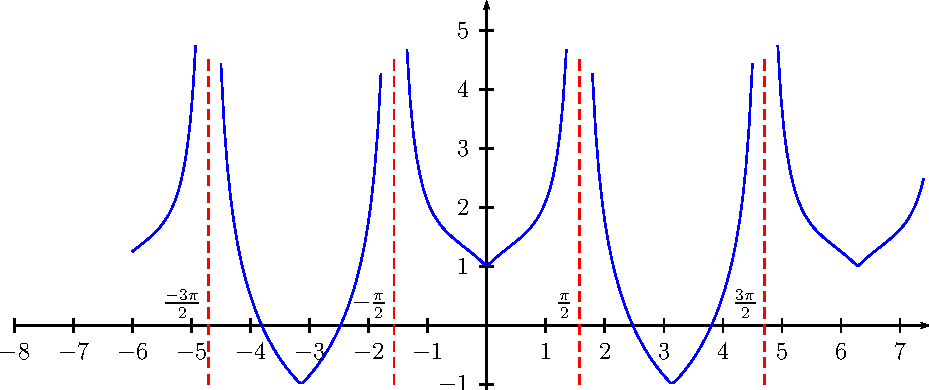
\includegraphics{../images/img005102-4}$$}
    \item \question{(***) $f_5(x)=\left(1+\frac{1}{x}\right)^x$ (à étudier sur $]0,+\infty[$).}
\reponse{Soit $x>0$. $x$ n'est pas nul donc $\frac{1}{x}$ existe puis $1+\frac{1}{x}>0$ et $f_6(x)$ existe.
\textbf{Etude en} $\bf{0.}$ Pour $x>0$, $x\ln(1+\frac{1}{x})=-x\ln x+x\ln(1+x)$. Par suite, $x\ln(1+\frac{1}{x})$ tend
vers $0$ quand $x$ tend vers $0$ par valeurs supérieures et donc $f_5(x)=\mbox{exp}(x\ln(1+\frac{1}{x}))$ tend vers
$1$.
Posons encore $f_5(0)=1$ et étudions la dérivabilité de $f_5$ en $0$. Pour $x>0$,

$$\frac{f_5(x)-f_5(0)}{x-0}=\frac{1}{x}\left(\text{exp}(x\ln(1+\frac{1}{x}))-1\right)
=\frac{\text{exp}\left(x\ln(1+\frac{1}{x})\right)-1}{x\ln\left(1+\frac{1}{x}\right)}\ln\left(1+\frac{1}{x}\right).$$
Or, $x\ln\left(1+\frac{1}{x}\right)$ tend vers $0$ quand $x$ tend vers $0$, et donc

$$\lim_{\substack{x\rightarrow0\\
x>0}}\frac{\mbox{exp}(x\ln\left(1+\frac{1}{x})\right)-1}{x\ln\left(1+\frac{1}{x}\right)}=\lim_{y\rightarrow 0}\frac{e^y-1}{y}=1.$$
D'autre part, $\ln\left(1+\frac{1}{x}\right)$ tend vers $+\infty$ quand $x$ tend vers $0$ par valeurs supérieures. Finalement,

$$\lim_{\substack{x\rightarrow0\\
x>0}}\frac{f_5(x)-f_5(0)}{x-0}=+\infty.$$
Ainsi, $f_5$ n'est pas dérivable en $0$ mais $\mathcal{C}_5$ admet l'axe des ordonnées pour tangente en
$(0,f_5(0))=(0,1)$.
\textbf{Etude en} $+\infty.$ Pour $x>0$,
$x\ln\left(1+\frac{1}{x}\right)=\frac{\ln\left(1+\frac{1}{x}\right)}{\frac{1}{x}}$ et 
donc $\lim_{x\rightarrow +\infty}x\ln\left(1+\frac{1}{x}\right)=\lim_{y\rightarrow 0}\frac{\ln(1+y)}{y}=1$.
Par suite,

$$\lim_{x\rightarrow +\infty}f_5(x)=e.$$
\textbf{Etude des variations de} $\bf{f_5.}$ Pour $x>0$, $f_5(x)>0$ puis $\ln(f_5(x))=x\ln(1+\frac{1}{x})$. Par suite,
pour $x>0$,

$$f_5'(x)=f_5(x)\ln(f_5)'(x)=f_5(x)\left(\ln\left(1+\frac{1}{x}\right)+\frac{x(-\frac{1}{x^2})}{1+\frac{1}{x}}\right)=f_5(x)g(x),$$
où $g(x)=\ln\left(1+\frac{1}{x}\right)-\frac{1}{1+x}$. Sur $]0,+\infty[$, $f_5'$ est du signe de $g$.
Pour déterminer le signe de $g$, étudions d'abord les variations de $g$ sur $]0,+\infty[$. $g$ est dérivable sur
$]0,+\infty[$ et pour $x>0$,

$$g'(x)=\frac{-\frac{1}{x^2}}{1+\frac{1}{x}}+\frac{1}{(x+1)^2}=-\frac{1}{x(x+1)}+\frac{1}{(x+1)^2}
=\frac{-1}{x(x+1)^2}<0.$$
$g$ est donc strictement décroissante sur $]0,+\infty[$, et puisque $\lim_{x\rightarrow +\infty}g(x)=0$, $g$ est strictement
positive sur $]0,+\infty[$. Il en est de même de $f_5'$. $f_5$ est strictement croissante sur $]0,+\infty($.
On en déduit $\mathcal{C}_5$.

$$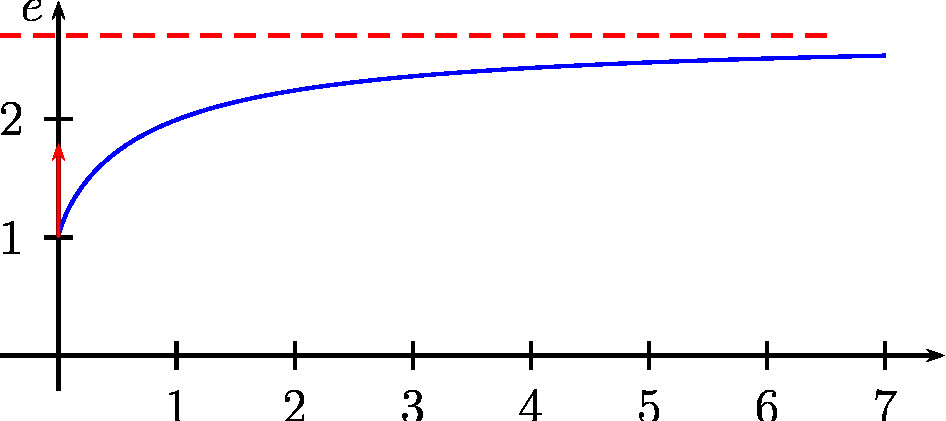
\includegraphics{../images/img005102-5}$$}
    \item \question{(**) $f_6(x)=\mbox{log}_2(1-\mbox{log}_{\frac{1}{2}}(x^2-5x+6))$.}
\reponse{\textbf{Domaine de définition de} $\bf{f_6.}$ Soit $x\in\Rr$.

\begin{align*}
f_6(x)\;\mbox{existe}&\Leftrightarrow x^2-5x+6>0\;\mbox{et}\;1-\mbox{log}_{\frac{1}{2}}(x^2-5x+6)>0
\Leftrightarrow x^2-5x+6>0\;\mbox{et}\;\frac{\ln(x^2-5x+6)}{\ln\frac{1}{2}}<1\\
 &\Leftrightarrow x^2-5x+6>0\;\mbox{et}\;\ln(x^2-5x+6)>\ln\frac{1}{2}\Leftrightarrow x^2-5x+6>\frac{1}{2}\\
 &\Leftrightarrow x^2-5x+\frac{11}{2}>0\Leftrightarrow x\in]-\infty,\frac{5-\sqrt{3}}{2}[\cup]\frac{5+\sqrt{3}}{2},+\infty[=\mathcal{D}_f.
\end{align*}
\textbf{Variations de} $\bf{f_6.}$ La fonction $x\mapsto x^2-5x+6$ est strictement décroissante sur
$\left]-\infty,\frac{5}{2}\right]$ et strictement croissante sur $\left[\frac{5}{2},+\infty\right[$. Comme
$\frac{5+\sqrt{3}}{2}>\frac{5}{2}$ et que $\frac{5-\sqrt{3}}{2}<\frac{5}{2}$, la fonction $x\mapsto x^2-5x+6$ est
strictement décroissante sur$\left]-\infty,\frac{5-\sqrt{3}}{2}\right]$ et strictement croissante sur
$\left[\frac{5+\sqrt{3}}{2},+\infty\right[$, à valeurs dans $]0,+\infty[$, intervalle sur lequel la fonction logarithme néperien
est strictement croissante. La fonction $x\mapsto1+\frac{\ln(x^2-5x+6)}{\ln2}$ a le même sens de variations et
finalement $f_6$ est strictement décroissante sur $\left]-\infty,\frac{5-\sqrt{3}}{2}\right]$ et strictement croissante
sur $\left[\frac{5+\sqrt{3}}{2},+\infty\right[$.
\textbf{Axe de symétrie} Soit $x\in\Rr$. $x\in\mathcal{D}_f\Leftrightarrow\frac{5}{2}-x\in\mathcal{D}_f$ et de 
plus, $\left(\frac{5}{2}-x\right)^2-5\left(\frac{5}{2}-x\right)+6=x^2-5x+6$. Par suite,

$$\forall x\in D,\;f_6(\frac{5}{2}-x)=f_6(x).$$

$\mathcal{C}_6$ admet donc la droite d'équation $x=\frac{5}{2}$ pour axe de symétrie.

Le calcul des limites étant immédiat, on en déduit $\mathcal{C}_6$.

$$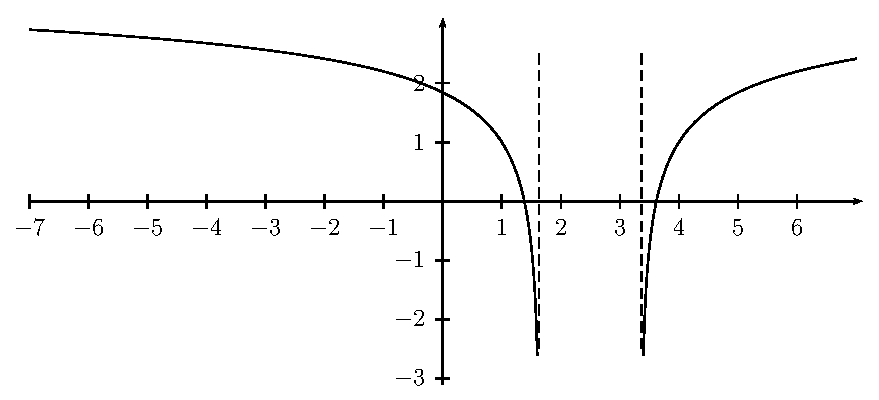
\includegraphics{../images/img005102-6}$$}
\end{enumerate}
}
